% This is samplepaper.tex, a sample chapter demonstrating the
% LLNCS macro package for Springer Computer Science proceedings;
% Version 2.20 of 2017/10/04
%
\documentclass[runningheads]{llncs}
%
\usepackage{graphicx}
\usepackage{algorithm}
\usepackage{algorithmic}
\usepackage{subfigure}
\usepackage{url}
\usepackage{amsmath}
% Used for displaying a sample figure. If possible, figure files should
% be included in EPS format.
%
% If you use the hyperref package, please uncomment the following line
% to display URLs in blue roman font according to Springer's eBook style:
% \renewcommand\UrlFont{\color{blue}\rmfamily}

\begin{document}
%
\title{Niche Radius adaptation in Bat Algorithm for Capturing Multiple Global Optima in Multimodal Functions 
% \thanks{Supported by organization x.}
}
%
%\titlerunning{Abbreviated paper title}
% If the paper title is too long for the running head, you can set
% an abbreviated paper title here
%
% \author{First Author\inst{1}\orcidID{0000-1111-2222-3333} \and
% Second Author\inst{2,3}\orcidID{1111-2222-3333-4444} \and
% Third Author\inst{3}\orcidID{2222--3333-4444-5555}}
%
% \authorrunning{F. Author et al.}
% First names are abbreviated in the running head.
% If there are more than two authors, 'et al.' is used.
%
% \institute{Princeton University, Princeton NJ 08544, USA \and
% Springer Heidelberg, Tiergartenstr. 17, 69121 Heidelberg, Germany
% \email{lncs@springer.com}\\
% \url{http://www.springer.com/gp/computer-science/lncs} \and
% ABC Institute, Rupert-Karls-University Heidelberg, Heidelberg, Germany\\
% \email{\{abc,lncs\}@uni-heidelberg.de}}
%
\maketitle              % typeset the header of the contribution
%
\begin{abstract}
% The abstract should briefly summarize the contents of the paper in
% 150--250 words.
    This paper proposes the niche radius-based bat algorithm (NRBA), which is designed to find multiple local optima in multimodal optimization.
    We focus on bat algorithm (BA) which deals with the trade-off between exploration and exploitation in the evolutionary process and extend it with niche radius which can control and modify the search space of solutions to avoid overlapping the found optima. In detail, the proposed BA is consist of three search phases: (i) the movement from neighbors for avoiding overlapping the same found optima; (ii) the exploitation for searching nearby the best solution of its domain with Niche Radius; (iii) the exploration for searching randomly in all domain of the radius. In order to evaluate the performance of NRBA, this paper employs some test-bed multimodal functions and compare NRBA with BA. The experimental results suggest that NRBA is able to provide the better search performance than BA to find multiple global optima in most of best-bed multimodal functions.

\keywords{Bat Algorithm  \and Multimodal Optimization \and Swarm Intelligence}
\end{abstract}
%
%
%
\section{Introduction}
There are many studies on evolutionary algorithms (EAs) solving the real-world optimization problems which are mostly multimodal and complex optimization problems. These problems has not only single global optimum but also many local optima, hence EAs are required to find the both multiple optima which might be changed their own location as the environment changes. 
% However, most of EAs such as Genetic Algorithm (GA) \cite{GA}, Particle Swarm Optimization (PSO) \cite{PSO01} and Differential Evolution(DE) \cite{DE} designed to converge toward a single global optimum for the static environment, is difficult to find these optima.

To tackle multimodal optimization problems, numerous techniques which are commonly known as \textit{niching methods} have proposed in \cite{Niching}-\cite{EAs02}, \cite{CDE} \cite{SDE}. Thomsen proposed the DE \cite{DE} extends with a crowding scheme (CDE) \cite{CDE} to replace the high-quality solution by the most similar candidate solutions. Li proposed the DE with Speciation (SDE) \cite{SDE} to keep a solution away from the nearest neighbor solution when the distance of both these solutions is less than the threshold. However, these niching methods are still not enough to find multiple local optima because both of them do not consider searching globally though they consider the solution movement according to the euclidean distance between the nearest neighbor solutions. For solving this problem, this paper focuses on Bat Algorithm (BA) that has the characteristic of echolocation which can predict the distance between bats and the target (\textit{i.e., object/food source}). This algorithm enables bats to estimate the distance between their location and the target even in the situations such as the target surrounded by obstacles and the absence of light. Bats can adjust their velocity which is controlled by their loudness, pulse emission rate and frequency, toward the target. While the iteration search step continues until bats reaches the target in the evolutionary process, bats will stop searching the target within its perceptible distance. This research employs BA which copes with exploitation and exploration search, extending with Niche Radius for multimodal optimization. Niche Radius is the threshold distance calculated by the fitness landscape and the number of its peaks.
% In this research, BA is employed because of the following reasons: (1) BA based on the three search phases from (i) to (iii) as described above, while EAs are mainly based on one search phase; and (2) this difference suggests that one of search phases in BA can be modified for finding multiple local optima with keeping the two search phases as original, while the search phase in EAs are hard to be modified for such a purpose due to a lack of the original search phase. What should be noted here is that BA still has the functions of exploitation and exploration in the solution search process as a local search by the phase (ii) and a global search by the phase (iii). Additionally, we extend BA with Niche Radius, which can control and separate the search space of solutions to avoid overlapping the found optima. Niche Radius ***.

This paper is organized as follows. After this section, the mechanism of BA and the proposed algorithm NRBA are explained in Sections 2 and 3. Section 4 describes the multimodal functions as the test-bed problem in the experiment. Section 5 shows the results while Section 6 discusses them. Finally, this paper concludes in Section 7.

\section{Bat Algorithm}
As mentioned in Section 1, BA is a metaheuristic algorithm based on the bat behavior according to its loudness and pulse emission rate of the reflect wave, which control the balance between a local and global search. When a bat finds the better solution than the current one, the loudness $A_i$ and the pulse rate $r_i$ gradually decreases and increases, respectively. To find better solution, the bat has the following three solution search phases: (i) the bat $i$ flies to the target (\textit{i.e.}, the bat which finds the best solution) with the velocity controlled by frequency $f_i$; (ii) the bat $i$ flies around the target as a local search; and (iii) the bat $i$ flies randomly in search space as a global search.
Let us explain these search phases.
First, in the search phase (i), all bats change their locations $x_i$ with their velocities $v_i$ toward the global best solution. For this calculation, the frequency $f_i$, velocity $v_i$, and location $x_i$, of the bat $i$ are calculated as follows:
\begin{equation}
f_{i} =f_{min}+(f_{max}-f_{min}) \beta
\label{eq:freq} 
\end{equation}

\begin{equation}
v_i^{t+1}=v_i^t+(x_*-x_i^t)* f_i
\label{eq:vi}
\end{equation}
\begin{equation}
x_i^{t+1}=x_i^t+v_i^{t+1}
\label{eq:xi}
\end{equation}
In detail, the new solution $x_i$ is updated by adding the new the velocity ${v_i}$ which is derived from the previous velocity $v_i^t$, the distance between the global best location and the previous location $(x_*-x_i^t)$, and frequency $f_i$ which range is [${f_{min}}$, ${f_{max}}$] where ${f_{min}}=0$ and ${f_{max}}=1$. $\beta $ is uniform random value from 0 to 1. Next, in the solution search phase (ii), the new solution $x_{loc}$ is generated around the global best solution as follows:
\begin{equation}
x_{loc}=x_{*}+ \epsilon A^t \ ,
\label{eq:loc}
\end{equation}
where ${\epsilon}$ is uniform random value between ${[0,  \ 1]}$. In Eq.(\ref{eq:A}), ${A^t}$ is the averaged loudness of all bats. Finally, in the search phase (iii), $x_{rnd}$ is generated randomly in search space as follows:
\begin{equation}
\label{eq:xrnd}
x_{rnd}=x_{lb}+(x_{ub}-x_{lb})*rand(1,D)
\end{equation}
where $x_{ub}$ and $x_{lb}$ describe the upper and lower bounds of the search space, and $rand(1,D)$ is the $D$ dimensional uniform random value between $[0, \ 1]$. 

When a bat finds the better solution than the current one, the loudness $A_i$ and pulse emission rate $r_i$ are updated as follows:
\begin{equation}
A_i^{t+1}=\alpha A_i^t
\label{eq:A}
\end{equation}
\begin{equation}
r_i^{t+1}=r_i^0[1-exp(-\gamma t)]
\label{eq:r}
\end{equation}
Note that the loudness $A_i^0$ is initialized as $A_i^0=1$ and the pulse rate is initialized as a uniform random value $r^0$ between $[0, \ 1]$ or a number closed around zero. The parameters $\alpha$ and $\gamma$ are the symbolized damping coefficient. The pseudo code of BA is given in the Algorithm 1 and its brief summary is described below.

\begin{itemize}
\item STEP1: Population initialization of bats (line 1 to 3)\\
The population of bats ${x_i}(i=1, 2, ..., N)$, the loudness ${A_i^0}$, the pulse rate ${r_i^0}$ are initialized as the initial values. The frequency ${f_i}$ is initialized by Eq.(\ref{eq:freq}).
\item STEP2: New solution updates (line 6)\\
The new solutions ${x_i}$ is calculated by Eqs. (\ref{eq:vi})(\ref{eq:xi}).
\item STEP3: New solution generation around global best solution ${x_*}$ (line 7 to 9)\\
A new solution $x_{loc}$ is generated around $x_*$ by Eq. (\ref{eq:loc}) when the pulse emission rate $r_i$ is lower than a random value.
\item STEP4: Random new solution generation (line 10)\\
A new solution ${x_{rnd}}$ is generated randomly by Eq. (\ref{eq:xrnd}).  
\item STEP5: Solutions update(line 11 to 14)\\
When ${rand < A_i}$, the best solution is selected from $x_i$, ${x_{loc}}$, and ${x_{rnd}}$ by Eqs.(\ref{eq:A}),(\ref{eq:r})
\item STEP6: Return to STEP2 
\end{itemize}

\begin{algorithm}[H]
\caption{Bat Algorithm}
\label{code:ba}
\begin{algorithmic}[1]
\REQUIRE Objective\ Function\ $F(x)$
\STATE Initialize Population $x_i(i=1,2,..., N)$ and $v_i$\\
\STATE Define frequency $f_i$ at location $x_i$ [eq.(\ref{eq:freq})]
\STATE Initialize pulse rates $r_i$, and loudness $A_i$
\WHILE{($t <$ Max number of iterations)}
\FOR{i=1 to N}
\STATE Generate a new solution $x_i$ and velocity $v_i$ [eqs.(\ref{eq:vi}) to (\ref{eq:xi})]
\IF{($rand>r_i$)}
\STATE Generate a new solution $x_{loc}$ around a global best solution $x_i$ [eq.(\ref{eq:loc})] 
% \ELSE
% \STATE Continue
\ENDIF
\STATE Generate a new solution $x_{rnd}$ randomly
\IF{($rand<A_i \& \min (F(x_i), F(x_{loc}), F(x_{rnd})<F(x_{i*})$)}
\STATE Accept the new solution, and update pulse rate $r_i$ \\ \& loudness $A_i$ [eqs. (\ref{eq:A})(\ref{eq:r})]  
\ENDIF
\STATE Evaluate all bats and select a best solution $x_*$ in the current solutions
\ENDFOR
\STATE t=t+1
\ENDWHILE
\end{algorithmic}
\end{algorithm}

\section{Proposed Algorithm}
\subsection{Niche Radius}
Niche Radius (NR) \cite{Niche}\cite{DNCMA} is one of niching techniques to determine the radius which is calculated by the number of local optima and the scale of the fitness landscape as follows:
\begin{equation}
\label{eq:lambda}
\lambda =\frac{1}{2} \sqrt{(x_{ub}-x_{lb})^2}
\end{equation}
\begin{equation}
\label{eq:NR}
NR=\frac{\lambda}{\sqrt[D]{q}},
\end{equation}
where the lower and upper bound values are $x_{ub}$ and $x_{lb}$ of the $D$-th dimensional search space,   and the number of local optima is $q$. Each domain of the radius as $NR$ is wrapping the local optimum to avoid converging same optima.

\subsection{Niche Radius-based Bat Algorithm}
As stated earlier, proposed algorithm is extended BA with the concept of Niche Radius which is able to locate many solutions without converging the found global best solutions within the domain of niche radius. This process is given by
\begin{equation}
\label{eq:nrvi}
v_i^{t+1}=v_i^t+(x_i^t-x_{NR*})*f_i
\end{equation}
\begin{equation}
\label{eq:nrxi}
x_i^{t+1}= \begin{cases}
x_i^t+v_i^{t+1} & (if \ d_i^t < NR) \\
x_i^t & (otherwise)
\end{cases}
\end{equation}
where $x_{NR*}$ is the best solution in the domain of niche radius and $d_i^t$ indicates the euclidean distance between the nearest neighbor solutions. Fig. \ref{fig:niche} provides an example to illustrate the solution movement to keep the solution $x_i$ from the best solution $x_{NR*}$ in the domain of the radius, where the red circle and the yellow star indicates solution $x_i$ and the best solution $x_{NR*}$. This figure shows the situation that the solutions $x_1, x_2 $ and $ x_3$ are located in the area of $x_{NR*}$ with the radius. In this case, these solutions are moved out from the area of the best solution $x_{NR*}$.

\begin{figure}[h]
\begin{center}
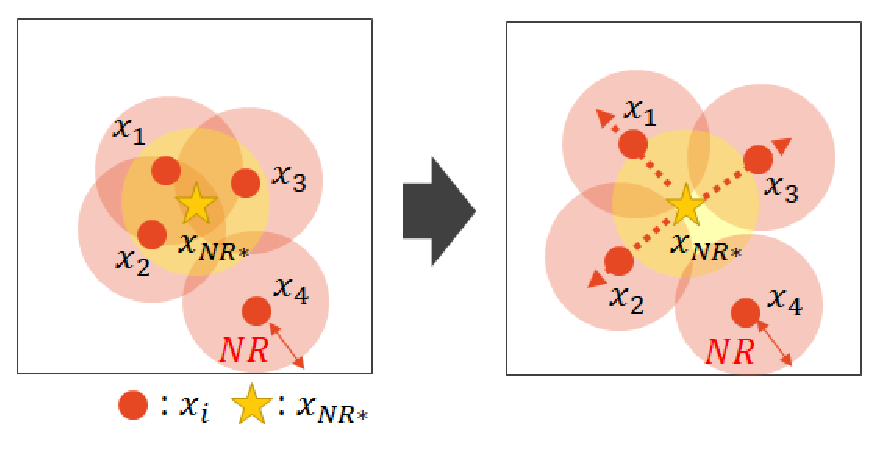
\includegraphics[width=0.8\linewidth]{eps/niche.eps}
\end{center}
\caption{Example of Solution Movement based on Niche Radius}
\label{fig:niche}
\end{figure}

In the local search phase, the new solution $x_{loc}$ is generated around the best solution $x_{NR*}$ in the domain of the radius as follows:
\begin{equation}
\label{eq:nrloc}
x_{loc}=x_{NR*} + \epsilon A_i^t
\end{equation}
where $A_i$ and $\epsilon$ is the same values as BA.
In the global search phase, the new solution $x_{rnd}$ is generated randomly in all domains of the range between $[-NR, NR]$ as follows: 
\begin{equation}
\label{eq:nrrnd}
x_{rnd}=x_i^t + rand(1,D,[-NR, NR])
\end{equation}

\subsection{Algorithm Description}
The pseudo code of NRBA is given in Algorithm 2 and its brief summary is described below.
\begin{algorithm}[H]
\caption{Niche Radius-based Bat Algorithm}
\label{code:ba}
\begin{algorithmic}[2]
\REQUIRE Objective\ Function\ $F(x)$
\STATE Initialize Population $x_i(i=1,2,..., N)$ and $v_i$\\
\STATE Define frequency $f_i$ at location $x_i$ [eq.(\ref{eq:freq})]
\STATE Initialize pulse rates $r_i$, and loudness $A_i$
\WHILE{($t <$ Max number of iterations)}
\FOR{i=1 to N}
\STATE Generate a new solution $x_i$ and velocity $v_i$ [eqs.(\ref{eq:nrvi}) to (\ref{eq:nrxi})]
\IF{($rand>r_i$)}
\STATE Generate a new solution $x_{loc}$ around a global best solution $x_i$ [eq.(\ref{eq:nrloc})] 
% \ELSE
% \STATE Continue
\ENDIF
\STATE Generate a new solution $x_{rnd}$ randomly [eq.(\ref{eq:nrrnd})]
\IF{($rand<A_i \& \min (F(x_i), F(x_{loc}), F(x_{rnd})<F(x_{i*})$)}
\STATE Accept the new solution, and update pulse rate $r_i$ \\ \& loudness $A_i$ [eqs. (\ref{eq:A})(\ref{eq:r})]  
\ENDIF
\STATE Evaluate all bats and select a best solution $x_*$ in the current solutions
\ENDFOR
\STATE t=t+1
\ENDWHILE
\end{algorithmic}
\end{algorithm}

\begin{itemize}
\item STEP1: Population initialization of bats (line 1 to 3)\\
The population of bats ${x_i}(i=1, 2, ..., N)$, the loudness ${A_i^0}$, the pulse rate ${r_i^0}$ are initialized as the initial values. The frequency ${f_i}$ is initialized by Eq.(\ref{eq:freq}).
\item STEP2: New solution updates (line 6)\\
The new solutions ${x_i}$ is calculated by Eqs. (\ref{eq:vi})(\ref{eq:xi}).
\item STEP3: New solution generation around global best solution ${x_*}$ (line 7 to 9)\\
A new solution $x_{loc}$ is generated around $x_*$ by Eq. (\ref{eq:loc}) when the pulse emission rate $r_i$ is lower than a random value.
\item STEP4: Random new solution generation (line 10)\\
A new solution ${x_{rnd}}$ is generated randomly by Eq. (\ref{eq:xrnd}).  
\item STEP5: Solutions update(line 11 to 14)\\
When ${rand < A_i}$, the best solution is selected from $x_i$, ${x_{loc}}$, and ${x_{rnd}}$ by Eqs.(\ref{eq:A}),(\ref{eq:r})
\item STEP6: Return to STEP2 
\end{itemize}

\section{Experimental Setup}
To measure the number of local optima and the convergence speed, we compare with the performance of all algorithms. In this section, four multimodal functions which are considered for maximization, are employed in \textit{Congress on Evolutionary Computation (CEC) 2013} competition \cite{cec2013}. 
\subsection{Benchmark Test Functions}
In order to verify the effectiveness of our proposed algorithm, four benchmark functions that are popular in multimodal optimization are employed in this experiments. The detail of these functions which are the search space, the fitness value of known global optima and the number of known global and local optima, are summarized in Table \ref{tab1}.


\begin{table}[h]
\caption{Measurement of Benchmark Test Functions}
\begin{center}
\begin{tabular}{c|c|c|c|c}
\hline
Function & ${F_1}$ & ${F_2}$ & ${F_3}$ & ${F_4}$ \\
\hline
Search Space & $x_1, x_2 \in [-6, \ 6]$ & $x_i \in [-10, \ 10]$ & $x_i \in [0.25, \ 10]$ & $x_i \in [0, \ 1]$\\
% & &  & & \\
\hline
Fitness Value & 200.0 & 186.731 & 1.0 & -2.0   \\
\hline
Number of global optima & 4 & 18 & 36 & 12 \\
\hline
Number of local optima &  0 & many & 0 & 0  \\
\hline
% \multicolumn{4}{l}{$^{\mathrm{a}}$Sample of a Table footnote.}
\end{tabular}
\label{tab1}
\end{center}
\end{table}

\begin{description}
\item[$F_1$: Himmelblau Function]\mbox{}\\
% This function is described as follows as shown in Fig. \ref{fig:3dgf}.
\begin{equation}
\label{eq:himmelblau}
F_1(x_1,x_2)=200-(x_1^2+x_2-11)^2+(x_1+x_2^2-7)^2
\end{equation}
The fitness value of the global optima is ${F(x_*)}=200$. This function has 4 global optima in the range between $x_1, x_2 \in [-6, \ 6]$.

\begin{figure}[h]
\begin{center}
\begin{tabular}{c}
\begin{minipage}{0.5\hsize}
\begin{center}
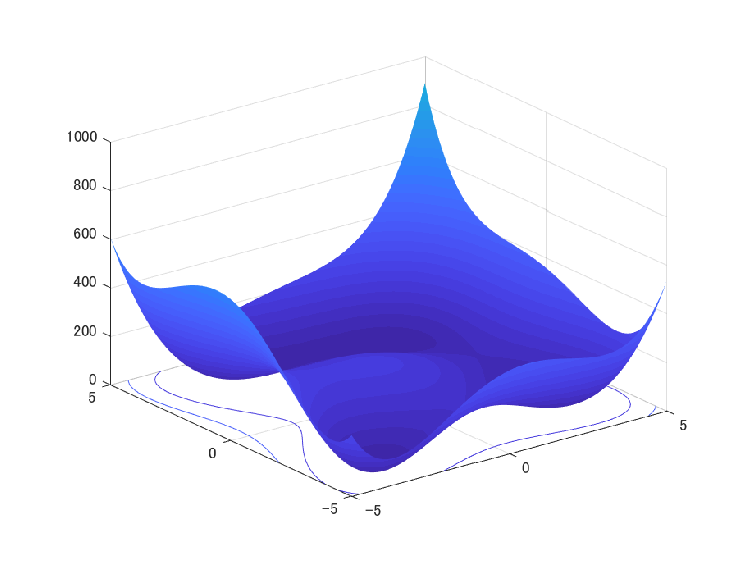
\includegraphics[width=1.0\linewidth]{eps/3d_himmelblau.eps}
\hspace{1.6cm} (a) The fitness landscape
\label{fig:3d_himmelblau}
\end{center}
\end{minipage}
\begin{minipage}{0.5\hsize}
\begin{center}
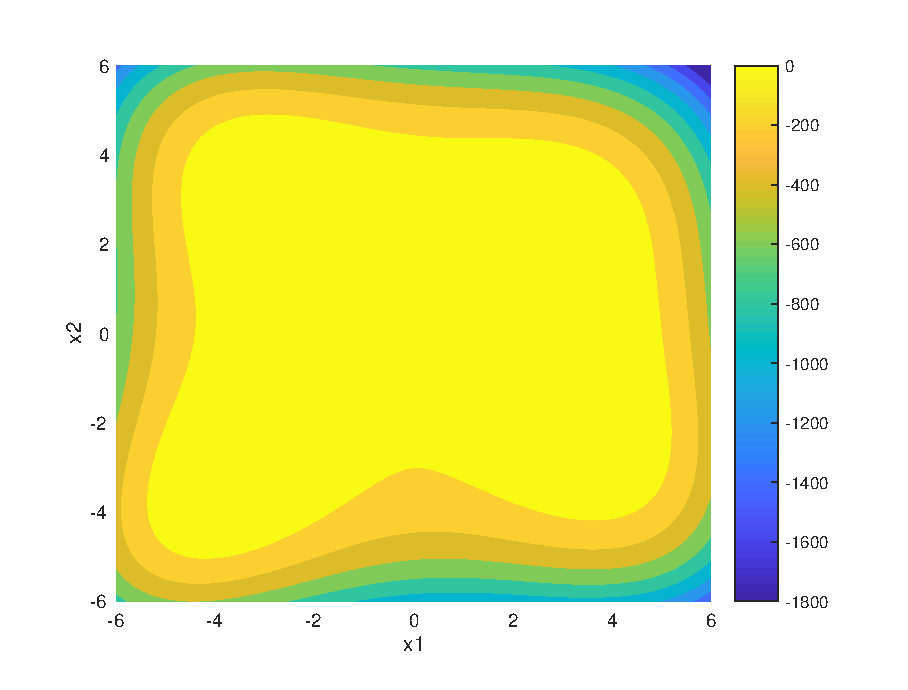
\includegraphics[width=1.0\linewidth]{eps/cont_himmelblau.eps}
\hspace{1.6cm} (b) The contour plot
\label{fig:cont_himmelblau}
\end{center}
\end{minipage}
\end{tabular}
\caption{Himmelblau}
\label{fig:f1}
\end{center}
\end{figure}

\item[$F_2$: Shubert Function]\mbox{}\\
 This function is described as follows as shown in Fig. \ref{fig:f2}.
 \begin{equation}
F_2(x) = -\prod_{i=1}^D \sum_{j=1}^5 j \cos[(j+1)x_i+j], 
\end{equation}
where $D$ is the number of dimension and the fitness value of the global optima is ${F(x_*)=187.731}$. This function has  $D \cdot 3^D $ global optima and numerous local optima in the range of search space between $x_i \in [-10, 10]^D$ with $i=1,2,...,D$. Fig. \ref{fig:f2} shows an example of the Shubert 2D function which has 18 global optima. 

\begin{figure}[h]
\begin{center}
\begin{tabular}{c}
\begin{minipage}{0.5\hsize}
\begin{center}
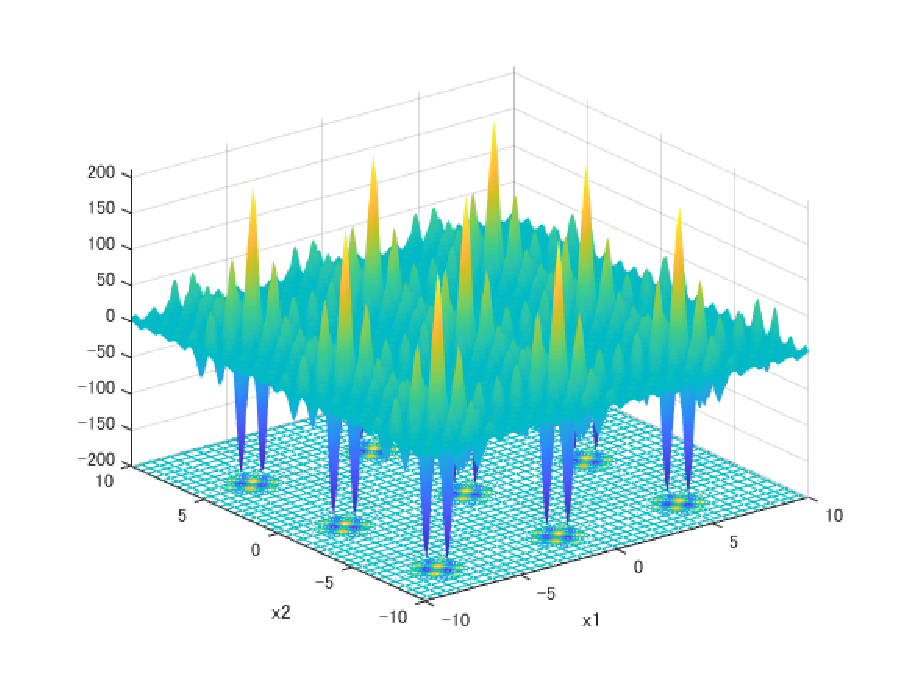
\includegraphics[width=1.0\linewidth]{eps/3d_shubert.eps}
\hspace{1.6cm} (a) The fitness landscape
\label{fig:3d_shubert}
\end{center}
\end{minipage}
\begin{minipage}{0.5\hsize}
\begin{center}
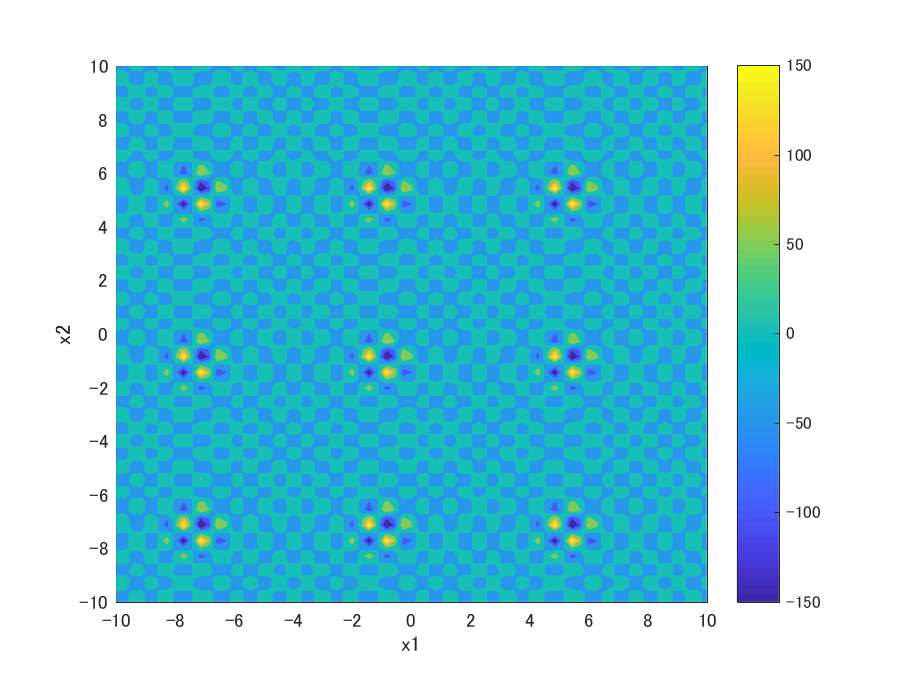
\includegraphics[width=1.0\linewidth]{eps/cont_shubert.eps}
\hspace{1.6cm} (b) The contour plot
\label{fig:cont_shubert}
\end{center}
\end{minipage}
\end{tabular}
\caption{Shubert}
\label{fig:f2}
\end{center}
\end{figure}

\item[$F_3$: Vincent Function]\mbox{}\\
 This function is described as follows as shown in Fig. \ref{fig:f3}.
 \begin{equation}
F_3(x) = \frac{1}{D} \sum_{i=1}^D \sin(10log(x_i)) 
\end{equation}
where $D$ is the number of the dimension and the fitness value of the global optima is ${F(x_*)=1.0}$. This function has $6^D $ global optima in the range of search space between $x_i \in [0.25, 10]^D$ with $i=1,2,...,D$. This figure provides the 2D function in case of 36 global optima with $D=2$. 

\begin{figure}[h]
\begin{center}
\begin{tabular}{c}
\begin{minipage}{0.5\hsize}
\begin{center}
\includegraphics[width=1.0\linewidth]{eps/3d_vincent.eps}
\hspace{1.6cm} (a) The fitness landscape
\label{fig:3d_vincent}
\end{center}
\end{minipage}
\begin{minipage}{0.5\hsize}
\begin{center}
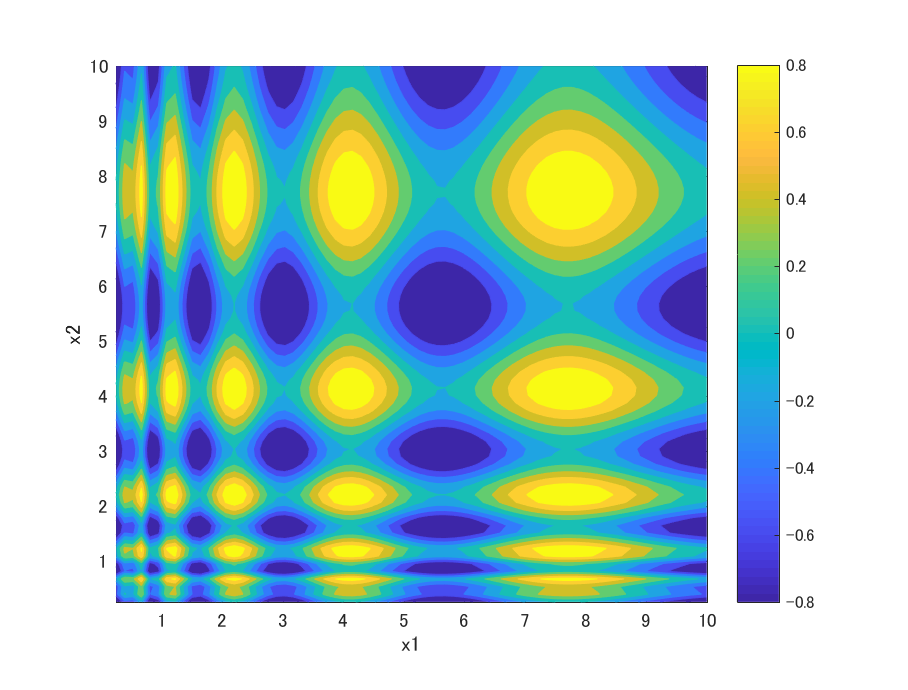
\includegraphics[width=1.0\linewidth]{eps/cont_vincent.eps}
\hspace{1.6cm} (b) The contour plot
\label{fig:cont_vincent}
\end{center}
\end{minipage}
\end{tabular}
\caption{Vincent}
\label{fig:f3}
\end{center}
\end{figure}

\item[$F_4$: Modified Rastrigin Function]\mbox{}\\
 This function is described as follows as shown in Fig. \ref{fig:f4}.
 \begin{equation}
F_4(x) = -\sum_{j=1}^D (10+9 \cos(2 \pi k_i x_i)) 
\end{equation}
where $D$ is the number of dimension and the fitness value of the global optima is ${f(x_*)=-2.0}$. In the case of $D=2$, this function has $\prod_{i=1}^D k_i$ \textit{(12 global optima)} with following setting: $k_1=k_3=1, k_2=4, k_=2$  global optima in the range of search space between $x_i \in [0, 1]^D$ with $i=1,2,...,D$.

\begin{figure}[h]
\begin{center}
\begin{tabular}{c}
\begin{minipage}{0.5\hsize}
\begin{center}
\includegraphics[width=1.0\linewidth]{eps/3d_rastrigin.eps}
\hspace{1.6cm} (a) The fitness landscape
\label{fig:3d_rastrigin}
\end{center}
\end{minipage}
\begin{minipage}{0.5\hsize}
\begin{center}
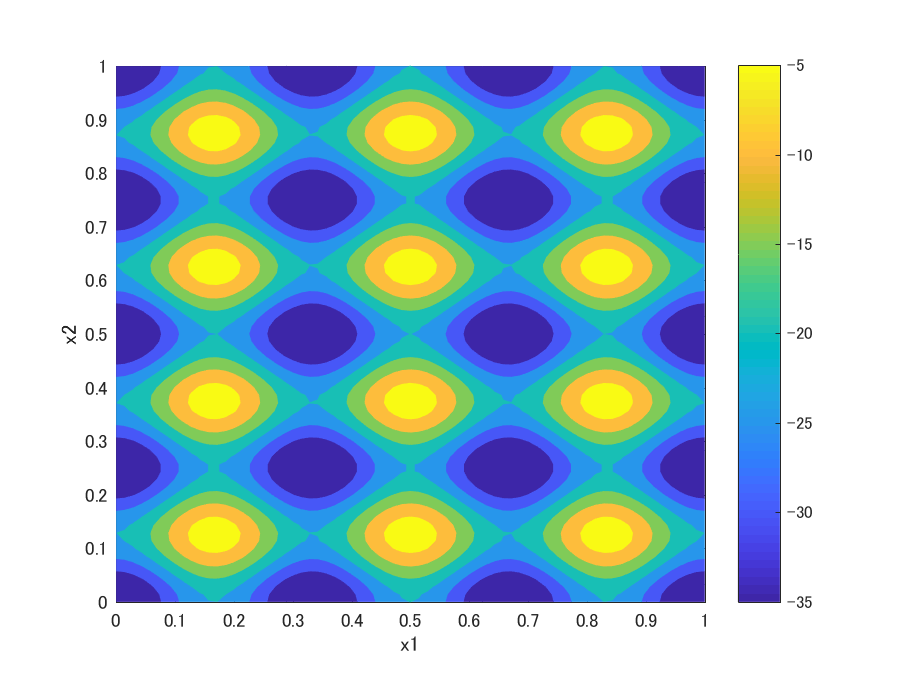
\includegraphics[width=1.0\linewidth]{eps/cont_rastrigin.eps}
\hspace{1.6cm} (b) The contour plot
\label{fig:cont_rastrigin}
\end{center}
\end{minipage}
\end{tabular}
\caption{Modified Rastrigin}
\label{fig:f4}
\end{center}
\end{figure}

\end{description}

\subsection{Performance Measurements}
\subsubsection{Peak Ratio}
This experiment employs Peak Ratio(PR) \cite{CDE} as the evaluation criterion in the CEC (IEEE Congress on Evolutionary Computation) 2013 competition \cite{cec2013}. The PR value measures the ratio of the found global and local optima in the total number of true peaks and it is calculated as follows: 
\begin{equation}
\label{eq:PR}
PR=\frac{\sum_{run=1}^{MR}FPs}{TP*MR}
\end{equation}
 where ${MR}$ indicates the maximum run, ${FPs}$ indicates indicates the number of peaks found by the optimization algorithm. ${TP}$ indicates the number of all known peaks of the function. We define that the peak is found when the Euclid distance between the all known peaks and the nearest solution calculated by the optimization algorithm is less than the thresholds $\varepsilon = \{1.0, 1.0E-1, 1.0E-2\}$.

\subsubsection{Peak Accuracy}
To measure how far solutions are close to the peaks, we employ Peak Accuracy (PA) \cite{CDE} calculated as follows:
\begin{equation}
PA=\sum_{j=1}^{TP}|F(s_j)-F(x_{NN_j})|,
\end{equation}
where $s_j$ and $x_{NN_j}$ denote the each known peak and the nearest neighbor solution. As the closest distance between both of them is short, the value of PA is close to 0.  

 \subsection{Experimental Parameters}
All experiments employ the parameters as follows: frequency ${f_{max}=1, f_{min}=0}$, loudness ${A^0}=1$, parse rate ${r^0} \in [0, \ 1]$ with ${\alpha =\gamma = 0.9}$. The population size ${N=100}$. This experiments are simulated 30 runs with different random seeds and 10000 evaluations as the termination condition for each run.

% \subsection{Comparison to other Algorithms}

\section{Results and Analysis}
To test the effectiveness of NRBA mechanism, this section investigates the peak ratio (PR) and the peak accuracy (PA) of each benchmark test function. Table \ref{tab2}, \ref{tab3}, and \ref{tab4} show the results that the PR and the PA values of two algorithms based on the settings of averaged over 30 individual runs at the final iteration. Fig. \ref{fig:results_ba} and \ref{fig:results_nrba} show that the solutions relocating and exploiting at the final iteration for all functions.

\begin{table}[h]
\caption{Peak Ratio and Peak Accuracy of BA and NRBA (averaged over 30 runs)}
\begin{center}
\begin{tabular}{c|c|c|c|c}
\multicolumn{5}{c}{$\varepsilon = 1.0$} \\
\hline
\multicolumn{1}{c|}{} & \multicolumn{2}{c|}{BA} & \multicolumn{2}{c}{NRBA} \\
\hline
 & PR & PA & PR & PA \\

Function & (Mean and SD) & (Mean and SD) & (Mean and SD) & (Mean and SD) \\
\hline
$F_1 $ & {\bf 1} $\pm$ 0 & {\bf 0.0060} $\pm$ 0.0028 & {\bf 1} $\pm$ 0  & 0.0326 $\pm$ 0.017  \\
\hline
$F_2 $ & 0.5870 $\pm$ 0.0991 & {\bf 3.9272} $\pm$ 1.199 & {\bf 0.7111} $\pm$ 0.1077 & 4.765 $\pm$ 1.3987 \\
\hline
$F_3 $ & 0.4407 $\pm$ 0.0839 & {\bf 0.0044} $\pm$ 0.0021 & {\bf 0.6685} $\pm$ 0.0699 & 0.0080 $\pm$ 0.0027 \\
\hline
$F_4 $ & 0.9833 $\pm$ 0.0333  & {\bf 0.0287} $\pm$ 0.0102 & {\bf 1} $\pm$ 0 & 0.029 $\pm$ 0.0097 \\
\hline
\end{tabular}
\label{tab2}
\end{center}
\end{table}

\begin{table}[h]
\caption{Peak Ratio and Peak Accuracy of BA and NRBA (averaged over 30 runs)}
\begin{center}
\begin{tabular}{c|c|c|c|c}
\multicolumn{5}{c}{$\varepsilon = 1.0E-1$} \\
\hline
\multicolumn{1}{c|}{} & \multicolumn{2}{c|}{BA} & \multicolumn{2}{c}{NRBA} \\
\hline
 & PR & PA & PR & PA \\

Function & (Mean and St. D.) & (Mean and St. D.) & (Mean and St. D.) & (Mean and St. D.) \\
\hline
$F_1 $ & {\bf 1} $\pm$ 0 & {\bf 0.0060} $\pm$ 0.0028 & {\bf 1} $\pm$ 0 & 0.0326 $\pm$ 0.0170  \\
\hline
$F_2 $ & 0.1148 $\pm$ 0.0640 & {\bf 0.0808} $\pm$ 0.0629 & {\bf 0.1185} $\pm$ 0.0821 & 0.1135 $\pm$ 0.0922 \\
\hline
$F_3 $ &  0.4407 $\pm$ 0.0839 & {\bf 0.0044} $\pm$ 0.0021 & {\bf 0.6685} $\pm$ 0.0699 & 0.0081 $\pm$ 0.0027\\
\hline
$F_4 $ & 0.9833 $\pm$ 0.0333 & {\bf 0.0287} $\pm$ 0.0102 & {\bf 1} $\pm$ 0 & 0.029 $\pm$ 0.0097 \\
\hline
\end{tabular}
\label{tab3}
\end{center}
\end{table}

\begin{table}[h]
\caption{Peak Ratio and Peak Accuracy of BA and NRBA (averaged over 30 runs)}
\begin{center}
\begin{tabular}{c|c|c|c|c}
\multicolumn{5}{c}{$\varepsilon = 1.0E-2$} \\
\hline
\multicolumn{1}{c|}{} & \multicolumn{2}{c|}{BA} & \multicolumn{2}{c}{NRBA} \\
\hline
 & PR & PA & PR & PA \\

Function & (Mean and St. D.) & (Mean and St. D.) & (Mean and St. D.) & (Mean and St. D.) \\
\hline
$F_1 $ & {\bf 1} $\pm$ 0 & {\bf 0.0060} $\pm$ 0.0028 & 0.6917 $\pm$ 0.3006 & 0.0127 $\pm$ 0.0076  \\
\hline
$F_2 $ & {\bf 0.0315} $\pm$ 0.04223 & 0.0029 $\pm$ 0.0040 & 0.0167 $\pm$ 0.0255 & {\bf 0.0020} $\pm$ 0.0034 \\
\hline
$F_3 $ & 0.4407 $\pm$ 0.0839 & {\bf 0.0044} $\pm$ 0.0021 & {\bf 0.6685} $\pm$ 0.0699 & 0.0078 $\pm$ 0.0031 \\
\hline
$F_4 $ & 0.9444 $\pm$ 0.0583 & {\bf 0.0215} $\pm$ 0.0069 & {\bf 0.9806} $\pm$ 0.0352 & 0.0234 $\pm$ 0.0074 \\
\hline
\end{tabular}
\label{tab4}
\end{center}
\end{table}

\begin{figure}[h]
\begin{tabular}{cc}
% \begin{center}

\renewcommand{\thefigure}{\alph{figure}}
\setcounter{figure}{0}
\begin{minipage}{0.5\hsize}
\centering
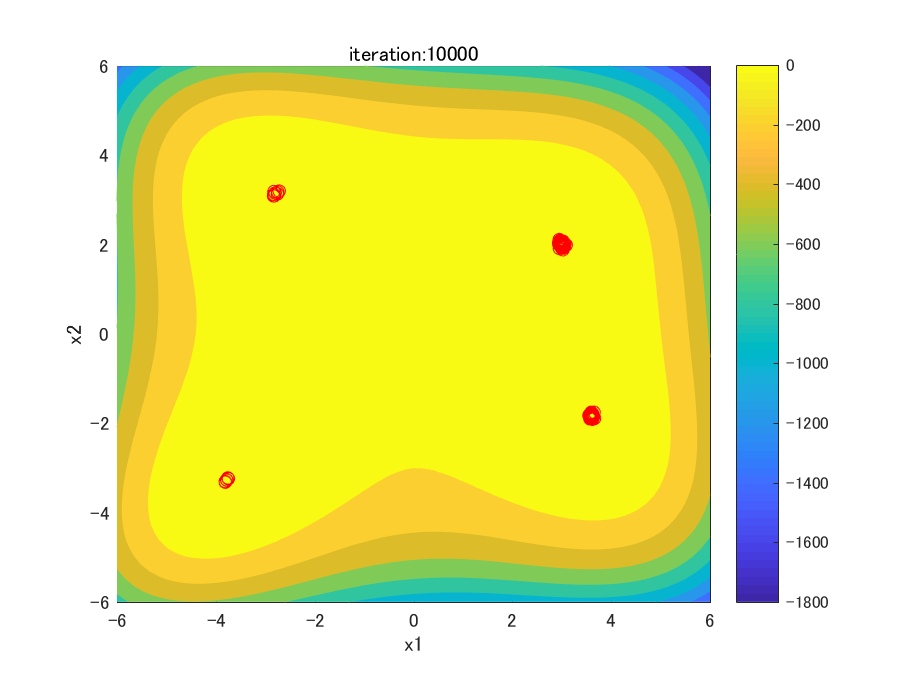
\includegraphics[width=1.0\linewidth]{eps/f1_ba.eps}

\caption{}
\label{fig:f1_ba}
\end{minipage} 

\begin{minipage}{0.5\hsize}
\centering
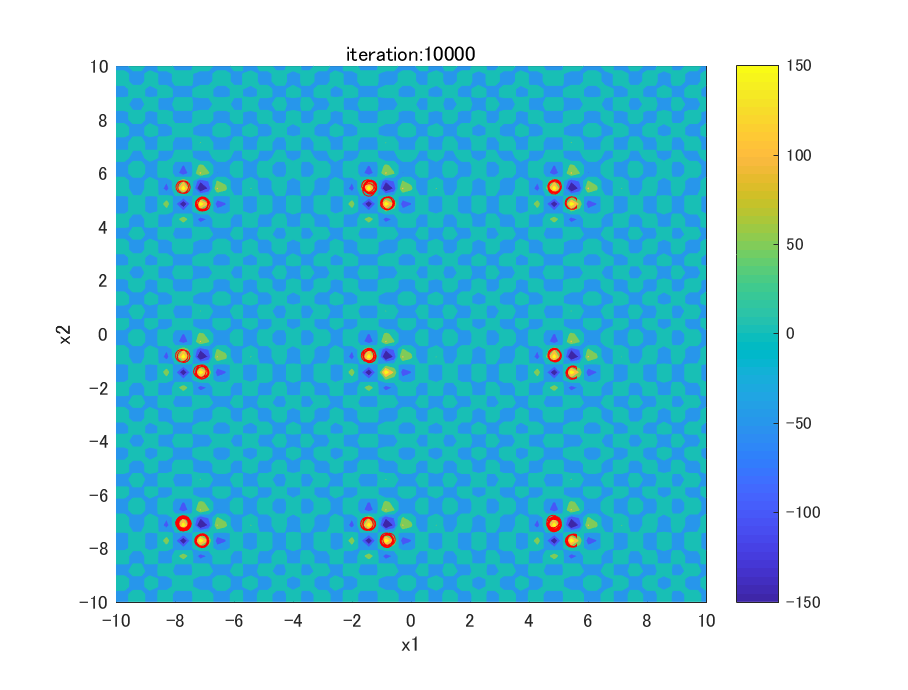
\includegraphics[width=1.0\linewidth]{eps/f2_ba.eps}
\caption{}
\label{fig:f2_ba}
\end{minipage} \\

\renewcommand{\thefigure}{\alph{figure}}
\begin{minipage}{0.5\hsize}
\centering
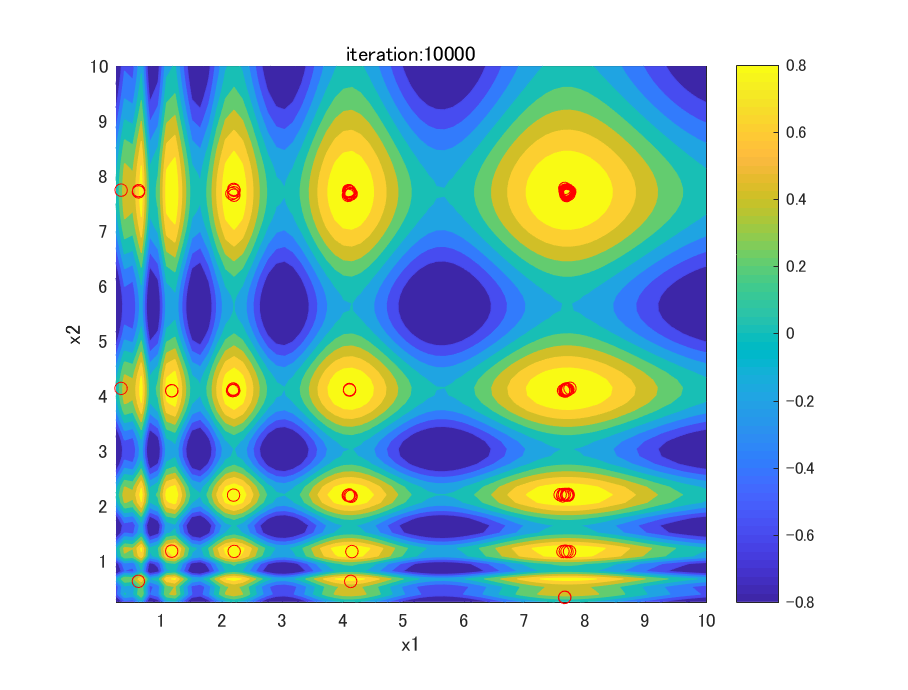
\includegraphics[width=1.0\linewidth]{eps/f3_ba.eps}
\caption{}
\label{fig:f3_ba}
\end{minipage} 

\begin{minipage}{0.5\hsize}
\centering
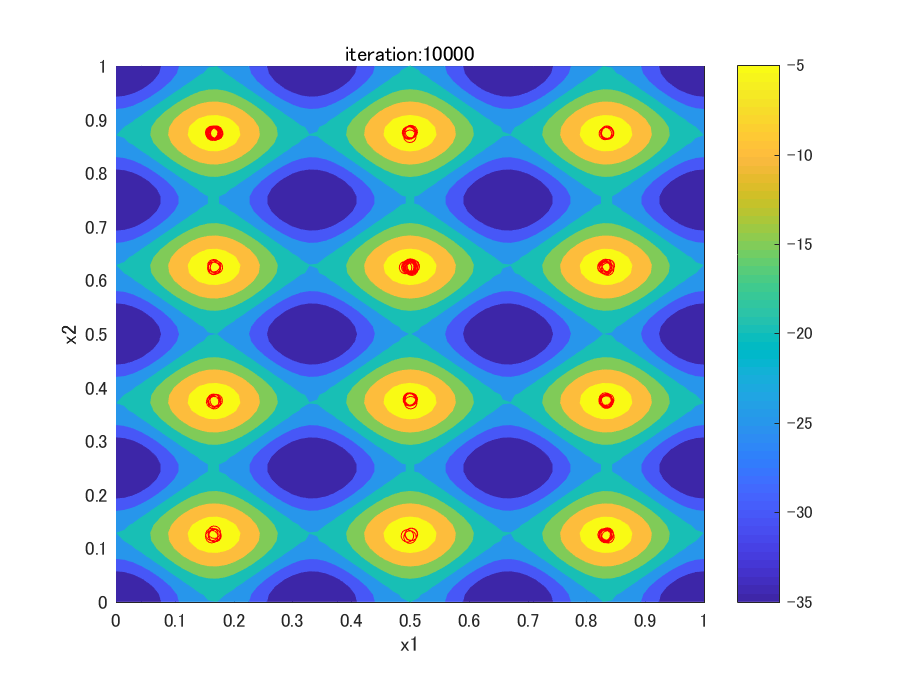
\includegraphics[width=1.0\linewidth]{eps/f4_ba.eps}
\caption{}
\label{fig:f4_ba}
\end{minipage}
\end{tabular}
\setcounter{figure}{5}
\caption{BA}
\label{fig:results_ba}
\end{figure}

\begin{figure}[h]
\begin{tabular}{cc}
\renewcommand{\thefigure}{\alph{figure}}
\setcounter{figure}{0}
\begin{minipage}{0.5\hsize}
\centering
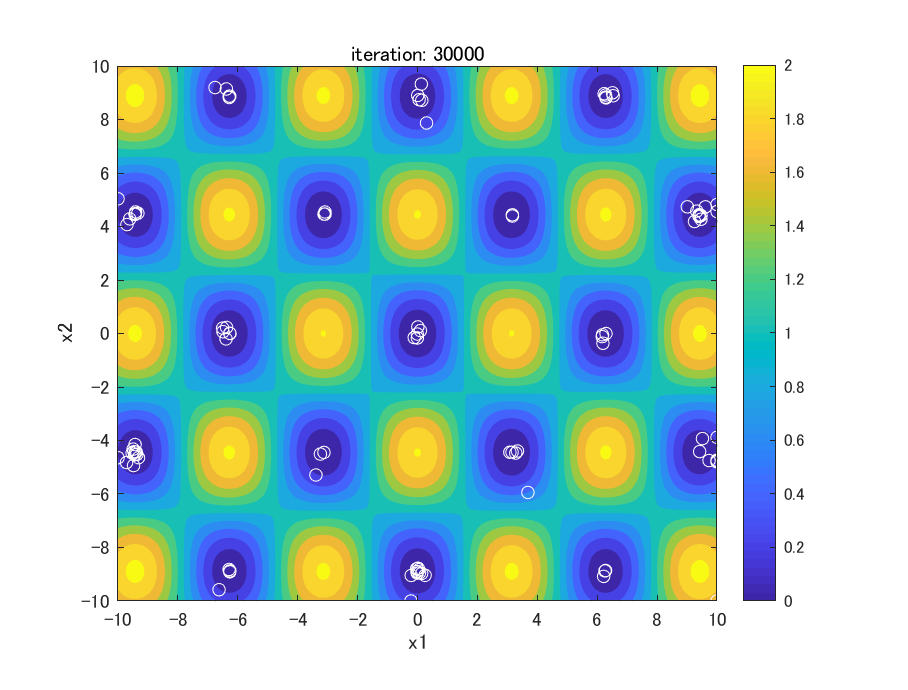
\includegraphics[width=1.0\linewidth]{eps/f1_nrba.eps}
\caption{}
\label{fig:f1_nrba}
\end{minipage} 

\begin{minipage}{0.5\hsize}
\centering
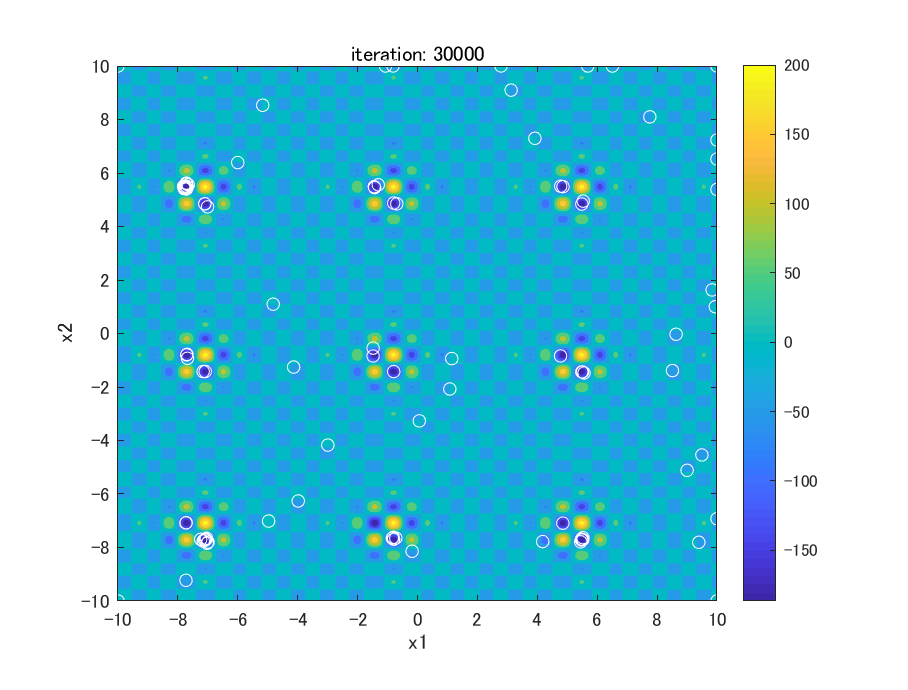
\includegraphics[width=1.0\linewidth]{eps/f2_nrba.eps}
\caption{}
\label{fig:f2_nrba}
\end{minipage} \\

\renewcommand{\thefigure}{\alph{figure}}
\begin{minipage}{0.5\hsize}
\centering
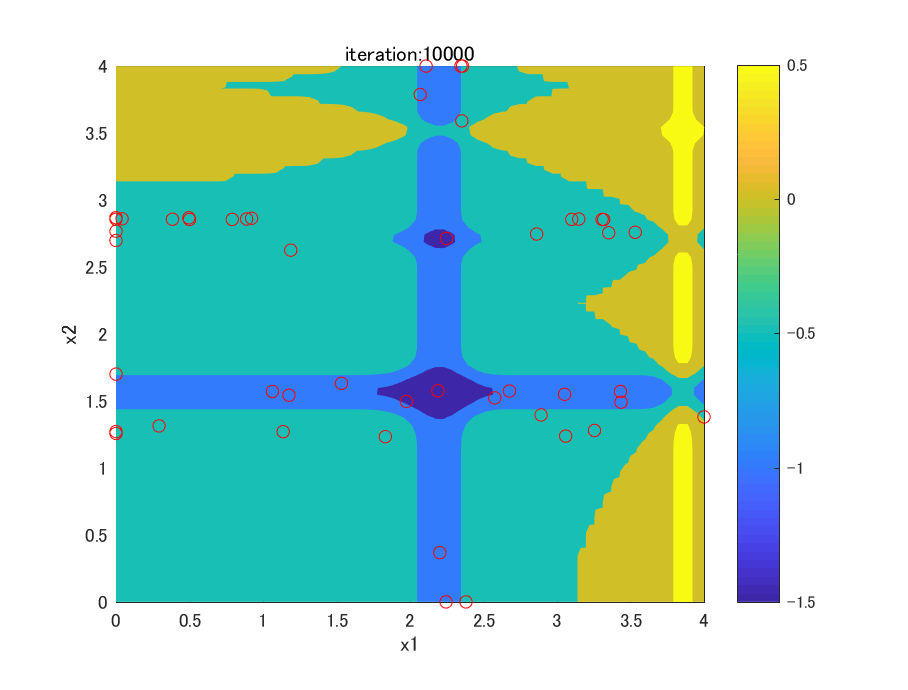
\includegraphics[width=1.0\linewidth]{eps/f3_nrba.eps}
\caption{}
\label{fig:f3_nrba}
\end{minipage} 

\begin{minipage}{0.5\hsize}
\centering
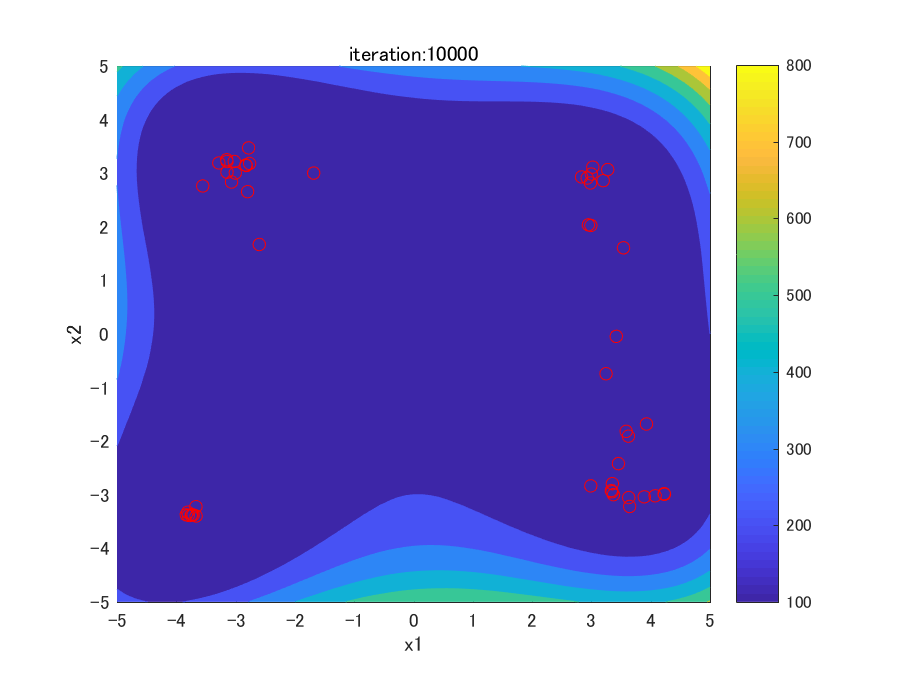
\includegraphics[width=1.0\linewidth]{eps/f4_nrba.eps}
\caption{}
\label{fig:f4_nrba}
\end{minipage} 

\end{tabular}
\setcounter{figure}{6}
\caption{NRBA}
\label{fig:results_nrba}

\end{figure}

\subsection{Peak Ratio}
From Table \ref{tab2} in the case of $\varepsilon = 1.0$, NRBA has outperformed than BA for all test functions. For $F_1$, the PR value of NRBA was the same as BA. It can see from this table, both algorithms are able to locate all global optima for all runs (as shown in Fig. \ref{fig:results_ba}-\ref{fig:f1_ba} and \ref{fig:results_nrba}-\ref{fig:f1_nrba}. The case of $\varepsilon=1.0E-1$ from Table \ref{tab3}, the PR values of NRBA were also higher than BA. However, the values of both algorithms went down greatly from Table \ref{tab2} to \ref{tab3} because $F_2$ is extremely sharp and complex landscape compared with the other functions. Table \ref{tab4} shows that NRBA has outperformed than BA in $F_3$ and $F_4$ in the case of $\varepsilon = 1.0E-2$. The performance of NRBA gradually decreased from Table \ref{tab2} to \ref{tab4}. As it can be seen in this table, NRBA was eventually worse than BA in $F_1$ and $F_2$. 

\subsection{Peak Accuracy}
NRBA is worse than BA for all functions from all Table \ref{tab2}, \ref{tab3} and \ref{tab4} except for $F_2$ in $\varepsilon=1.0E-2$. As it can be seen the results, the exploit phase of BA has worked well more than NRBA regardless of the difference value of threshold $\varepsilon$ from Table \ref{tab2}, \ref{tab3} and \ref{tab4}. Furthermore, the random search phase of BA is assumed to cope with the exploitation and the exploration. However, the density distribution of the solutions is unbalanced (especially in Fig. \ref{fig:results_ba}-\ref{fig:f1_ba} and \ref{fig:results_ba}-\ref{fig:f3_ba}) due to promoting all solutions to exploit the global best solution. In contrast, NRBA is able to spread the solutions to multiple optima even if some global optima are located the same domain of Niche Radius.

\section{Conclusion}
This paper proposes BA extending with Niche Radius which enables to avoid overlapping the solutions into the same peak and locate multiple global optima in several multimodal functions which are different from landscape and the number of peaks. For solving multimodal optimization, we improved the three search phases of BA: (i) the movement from neighbors for avoiding overlapping the same found optima; (ii) the exploitation for searching nearby the best solution of its domain with Niche Radius; (iii) the exploration for searching randomly in all domain of the radius. To evaluate the performance of NRBA, this algorithm were compared with BA. The results show that NRBA performed better than BA because the spatial distribution mechanism in NRBA copes with locating many multiple global optima. In contrast, BA is still better than NRBA regarding the peak accuracy which indicates how far the peaks are close to the solutions, due to the distribution mechanism of NRBA.

In the future, we will improve the algorithm performances: the exploration for searching all global optima completely, and the exploitation for locating global optima rapidly.
% \subsection{A Subsection Sample}
% Please note that the first paragraph of a section or subsection is
% not indented. The first paragraph that follows a table, figure,
% equation etc. does not need an indent, either.

% Subsequent paragraphs, however, are indented.

% \subsubsection{Sample Heading (Third Level)} Only two levels of
% headings should be numbered. Lower level headings remain unnumbered;
% they are formatted as run-in headings.

% \paragraph{Sample Heading (Fourth Level)}
% The contribution should contain no more than four levels of
% headings. Table~\ref{tab1} gives a summary of all heading levels.

% \begin{table}
% \caption{Table captions should be placed above the
% tables.}\label{tab1}
% \begin{tabular}{|l|l|l|}
% \hline
% Heading level &  Example & Font size and style\\
% \hline
% Title (centered) &  {\Large\bfseries Lecture Notes} & 14 point, bold\\
% 1st-level heading &  {\large\bfseries 1 Introduction} & 12 point, bold\\
% 2nd-level heading & {\bfseries 2.1 Printing Area} & 10 point, bold\\
% 3rd-level heading & {\bfseries Run-in Heading in Bold.} Text follows & 10 point, bold\\
% 4th-level heading & {\itshape Lowest Level Heading.} Text follows & 10 point, italic\\
% \hline
% \end{tabular}
% \end{table}


% \noindent Displayed equations are centered and set on a separate
% line.
% \begin{equation}
% x + y = z
% \end{equation}
% Please try to avoid rasterized images for line-art diagrams and
% schemas. Whenever possible, use vector graphics instead (see
% Fig.~\ref{fig1}).

% \begin{figure}
% 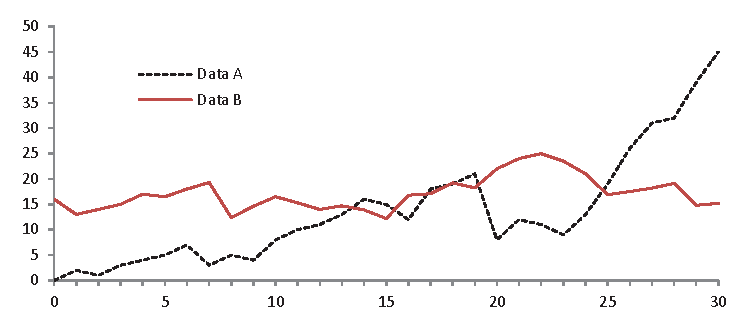
\includegraphics[width=\textwidth]{fig1.eps}
% \caption{A figure caption is always placed below the illustration.
% Please note that short captions are centered, while long ones are
% justified by the macro package automatically.} \label{fig1}
% \end{figure}

% \begin{theorem}
% This is a sample theorem. The run-in heading is set in bold, while
% the following text appears in italics. Definitions, lemmas,
% propositions, and corollaries are styled the same way.
% \end{theorem}
% %
% % the environments 'definition', 'lemma', 'proposition', 'corollary',
% % 'remark', and 'example' are defined in the LLNCS documentclass as well.
% %
% \begin{proof}
% Proofs, examples, and remarks have the initial word in italics,
% while the following text appears in normal font.
% \end{proof}
% For citations of references, we prefer the use of square brackets
% and consecutive numbers. Citations using labels or the author/year
% convention are also acceptable. The following bibliography provides
% a sample reference list with entries for journal
% articles~\cite{ref_article1}, an LNCS chapter~\cite{ref_lncs1}, a
% book~\cite{ref_book1}, proceedings without editors~\cite{ref_proc1},
% and a homepage~\cite{ref_url1}. Multiple citations are grouped
% \cite{ref_article1,ref_lncs1,ref_book1},
% \cite{ref_article1,ref_book1,ref_proc1,ref_url1}.
%
% ---- Bibliography ----
%
% BibTeX users should specify bibliography style 'splncs04'.
% References will then be sorted and formatted in the correct style.
%
% \bibliographystyle{splncs04}
% \bibliography{mybibliography}
%
\begin{thebibliography}{8}
\bibitem{Niching}
S. W. Mahfoud, A comparison of parallel and sequential niching methods, in \textit{Proc. 6th Int. Conf. Genet. Algorithms}, pp.136-143, 1995.

% \bibitem{GA}
% M. Srinivas, L. M. Patniak, Genetic Algorithms: A Survey, \textit{Computer}, Vol.27, No.6, 17-26, 1994.

\bibitem{EAs01}
G. Singh and K. Deb, Comparison of Multi-modal Optimization Algorithms Based on Evolutionary algorithms., \textit{In Proceedings of the 8th Annual Conference on Genetic and Evolutionary Computation.}, 1305-1312, 2006.
% \bibitem{PSO01}
% R. Eberhart, J. Kennedy: A New Optimizer Using Particle Swarm Theory,
% \textit{Proc. Sixth International Symposium on Micro Machine and Human Science (Nagoya, Japan), IEEE Service center, Pis-cataway, NJ}, No.~1, pp.~39--43, 1995.

\bibitem{GAS}
D. E. Goldberg and J. Richardson, Genetic Algorithms with Sharing for Multimodal Function Optimization, in \textit{Proc. Genetic Algorithms Their Applicat. Conf.,}, pp.41-49, 1987.

\bibitem{EAs02}
R. K. Ursem, Multinational evolutionary algorithms, in \textit{Proc. Congr.Evol. Comput.(CEC)}, vol.3., pp.1633-1640, 1999.

\bibitem{DE}
R. Storn, K. Price, Differential Evolution − A simple and efficient adaptive scheme for global optimization over continuous spaces, Journal of global optimization, Vol.11, No.4, 341-359, 1997.

\bibitem{CDE}
R. Thomsen,"Multimodal Optimization using Crowding-based Differential Evolution," {\it In the IEEE Congress on Evolutionary Computation,}2004. CEC2004, vol.2, pp. 1382-1389, 19-23 June, 2004.

\bibitem{SDE}
X. Li, Efficient Differential Evolution using Speciation for Multimodal Function Optimization, \textit{In Proceedings of the Conference on genetic and evolutionary computation}, (GECCO'05), 873-880, 2005. 

% \bibitem{FA01}
% X. S. Yang: Firefly Algorithms for Multimodal Optimization,
% \textit{in:Stochastic Algorithms: Foundations and Applications, SAGA}, Vol.~5792, pp.~169--178, 2009.

\bibitem{BA01}
X. S. Yang: A Metaheuristic Bat-Inspired Algorithm,
 \textit{in: Nature Inspired Cooperative Strategies for Optimization(NICSO 2010), Springer, Berlin}, Vol.~284, pp.~65--74, 2010.

\bibitem{Niche} D.Beasley, D.R. Bull, and R.R. Martin, "A sequantial niche technique for multimodal function optimization," {\it Evolutionary Computation}, vol. 1, no.2, pp. 101-125,1993.

\bibitem{DNCMA}
O. M. Shir, T. Back: Dynamic niching in evolution strategies with covariance matrix adaption. \textit{In: Proceedings of the 2005 Congress on Evolutionary Computation(CEC2005)}, Piscataway, NJ, USA, IEEE Press (2005)
% \bibitem{f1}
% M. Molga, and C. Smutnicki, Test functions for optimization needs (2005). Retrieved June 2013, from \url{http://www.zsd.ict.pwr.wroc.pl/files/docs/functions.pdf.}

% \bibitem{f2}
% H. Pohlheim, GEATbx Examples: Examples of Objective Functions (2005). Retrieved June 2013, from \url{http://www.geatbx.com/download/GEATbx_ObjFunExpl_v37.pdf.}


\bibitem{cec2013}
X. Li, A. Engelbrecht, and M. G. Epitropakis, "Benchmark Functions for CEC'2013 Special Session and Competition on Niching Methods for Multimodal Function Optimization", {\it Evol. Comput.} Mach. Learn. Group, RMIT University, Melbourne, VIC, Australia, Tech. Rep., 2013.
\end{thebibliography}
\end{document}
